% !TeX spellcheck = es_ES
%----------------------------------------------------------------------------------------
%	PACKAGES AND OTHER DOCUMENT CONFIGURATIONS
%----------------------------------------------------------------------------------------

\documentclass[fleqn,10pt]{SelfArx} % Document font size and equations flushed left
%\usepackage{chemmacros}
\usepackage{ifthen}
\usepackage{calc}
\usepackage{microtype}
\usepackage{ifpdf}
\usepackage[utf8]{inputenc}
\usepackage{amsmath, amsfonts, amssymb}
\usepackage{graphicx, xcolor}
\usepackage{booktabs}
\usepackage{fancyhdr}
\usepackage{lastpage}
\usepackage{titlesec}
\usepackage{titletoc}
\usepackage{enumitem}
\usepackage[version=3]{mhchem}
\usepackage{lipsum}
\usepackage{graphbox}
\usepackage{tabularx}
%----------------------------------------------------------------------------------------
%	COLUMNS
%----------------------------------------------------------------------------------------

\setlength{\columnsep}{0.55cm} % Distance between the two columns of text
\setlength{\fboxrule}{1pt} % Width of the border around the abstract

%----------------------------------------------------------------------------------------
%	COLORS
%----------------------------------------------------------------------------------------

\definecolor{color1}{RGB}{0,94,157} % Color of the article title and sections
\definecolor{color2}{RGB}{255,243,210} % Color of the boxes behind the abstract and headings

%----------------------------------------------------------------------------------------
%	HYPERLINKS
%----------------------------------------------------------------------------------------

\usepackage{hyperref} % Required for hyperlinks
\hypersetup{hidelinks,colorlinks,breaklinks=true,urlcolor=color2,citecolor=color1,linkcolor=color1,bookmarksopen=false,pdftitle={Title},pdfauthor={Author}}

%----------------------------------------------------------------------------------------
%	ARTICLE INFORMATION
%----------------------------------------------------------------------------------------

\JournalInfo{L. de Qu\'imica inorg\'anica II, No. 3, 2016-20} % Journal information
%\Archive{Additional note} % Additional notes (e.g. copyright, DOI, review/research article)

\PaperTitle{Isomer\'ia Geom\'etrica} % Article title

\Authors{Juan Barbosa{\color{color1}\textsuperscript{1}\textsuperscript{,2}*},
	Alejandro Camacho{\color{color1}\textsuperscript{1}\textsuperscript{,3}**}} %
%Authors
\affiliation{{\color{color1}\textsuperscript{1}}\textit{Departamento de Qu\'imica, Universidad de los Andes, Bogot\'a, Colombia}} % Author affiliation
\affiliation{{\color{color1}\textsuperscript{2}}\textit{Departamento de F\'isica, Universidad de los Andes, Bogot\'a, Colombia}} % Author affiliation
\affiliation{{\color{color1}\textsuperscript{3}}\textit{Departamento de	F\'isica, Universidad Nacional, Bogot\'a, Colombia}}
\affiliation{{\color{color1}*}\textbf{Email}: js.barbosa10@uniandes.edu.co} %
%Corresponding author
\affiliation{{\color{color1}**}\textbf{Email}: a.camacho10@uniandes.edu.co}
\Keywords{ Cinética, orden de reacción, pH, paso determinante de una reacción, Cromo.} %
%Keywords - if you don't want any simply remove all the text between the curly
%brackets
\newcommand{\keywordname}{Keywords} % Defines the keywords heading name

%----------------------------------------------------------------------------------------
%	ABSTRACT
%----------------------------------------------------------------------------------------
\Abstract
{
Se realiza la síntesis del compuesto diclorobis(etilendiamin)cobalto(III) en sus dos especies (cis y trans), obteniendo que la especie trans es significativamente mas estable dado no solo su formación sino el alto rendimiento considerando que el método de síntesis falla en la oxidación completa del cromo (II) a cromo (III), probándose esto con el lavado de metanol y que conversión entre isómeros se puede ver afectada por la humedad o la presencia de otros compuestos que puedan actuar como bases de lewis. En este punto se logra un ligera conversión del isómero trans al cis pero solo al grado de opacar el compuesto a un violeta muy tenue en el interior de los cristales.
}
%----------------------------------------------------------------------------------------

\begin{document}
	\flushbottom % Makes all text pages the same height
	\maketitle % Print the title and abstract box
	%\tableofcontents % Print the contents section
	\thispagestyle{empty} % Removes page numbering from the first page
	%----------------------------------------------------------------------------------------
	%	ARTICLE CONTENTS
	%----------------------------------------------------------------------------------------
	\section*{Introducci\'on}
	El  cobalto al igual que otros metales de transición tiene la tendencia de reducir su estabilidad a medida que aumenta el estado de oxidación en que se encuentra el elemento, sin embargo, para los estados (II) y (III) la energía es tan próxima que la estabilidad dependerá del entorno químico y los ligandos relacionados al metal, es un elemento ferromagnetico, que forma de sales en su estado de oxidación dos y su reducción a $\ce{Co^{0}}$ suele ser bastante desfavorable.
	\\
	Los complejos de $\ce{Co^{(III)}}$ han sido estudiados a lo largo de la historia y se encontraron en el nacimiento de la química de coordinación y hasta el momento todos lo complejos de $\ce{Co^{(III)}}$ conocidos tiene geometría octaédrica. El cobalto posee gran afinidad por aquellos ligandos dadores que actuan como bases de lewis en particular por aquellos que contiene nitrógeno. Para sintetiza compuestos octaédricos de cobalto suele partirse de sale del tipo $\ce{CoX_{2}}$ se produce la oxidación con oxigeno molecular en la presencia de los ligandos a adicionar, durante varias se mantiene el flujo de oxigeno constante y calentamiento.
	
	Compuestos octaedricos con ligandos Cl en su estructura suelen ser de gran interés puesto que estos pueden ser sustituidos con mediana facilidad por otros ligandos anionicos, dando versatilidad en la síntesis inorgánica. \cite{cotton}
	
	Según la literatura con metanol como solvente, la cantidad que se obtiene del isómero cis no es representativa en comparación con la cantidad del compuesto trans lo que se ve explicado por la menor energía y tensión presente en esta configuración y a su vez esta diferencia de energía explica que la preparación del cis aunque en principio sencilla no se allá logrado.
	
	\begin{scheme}[h]
        \centering
        \begin{tabular}{cc}
            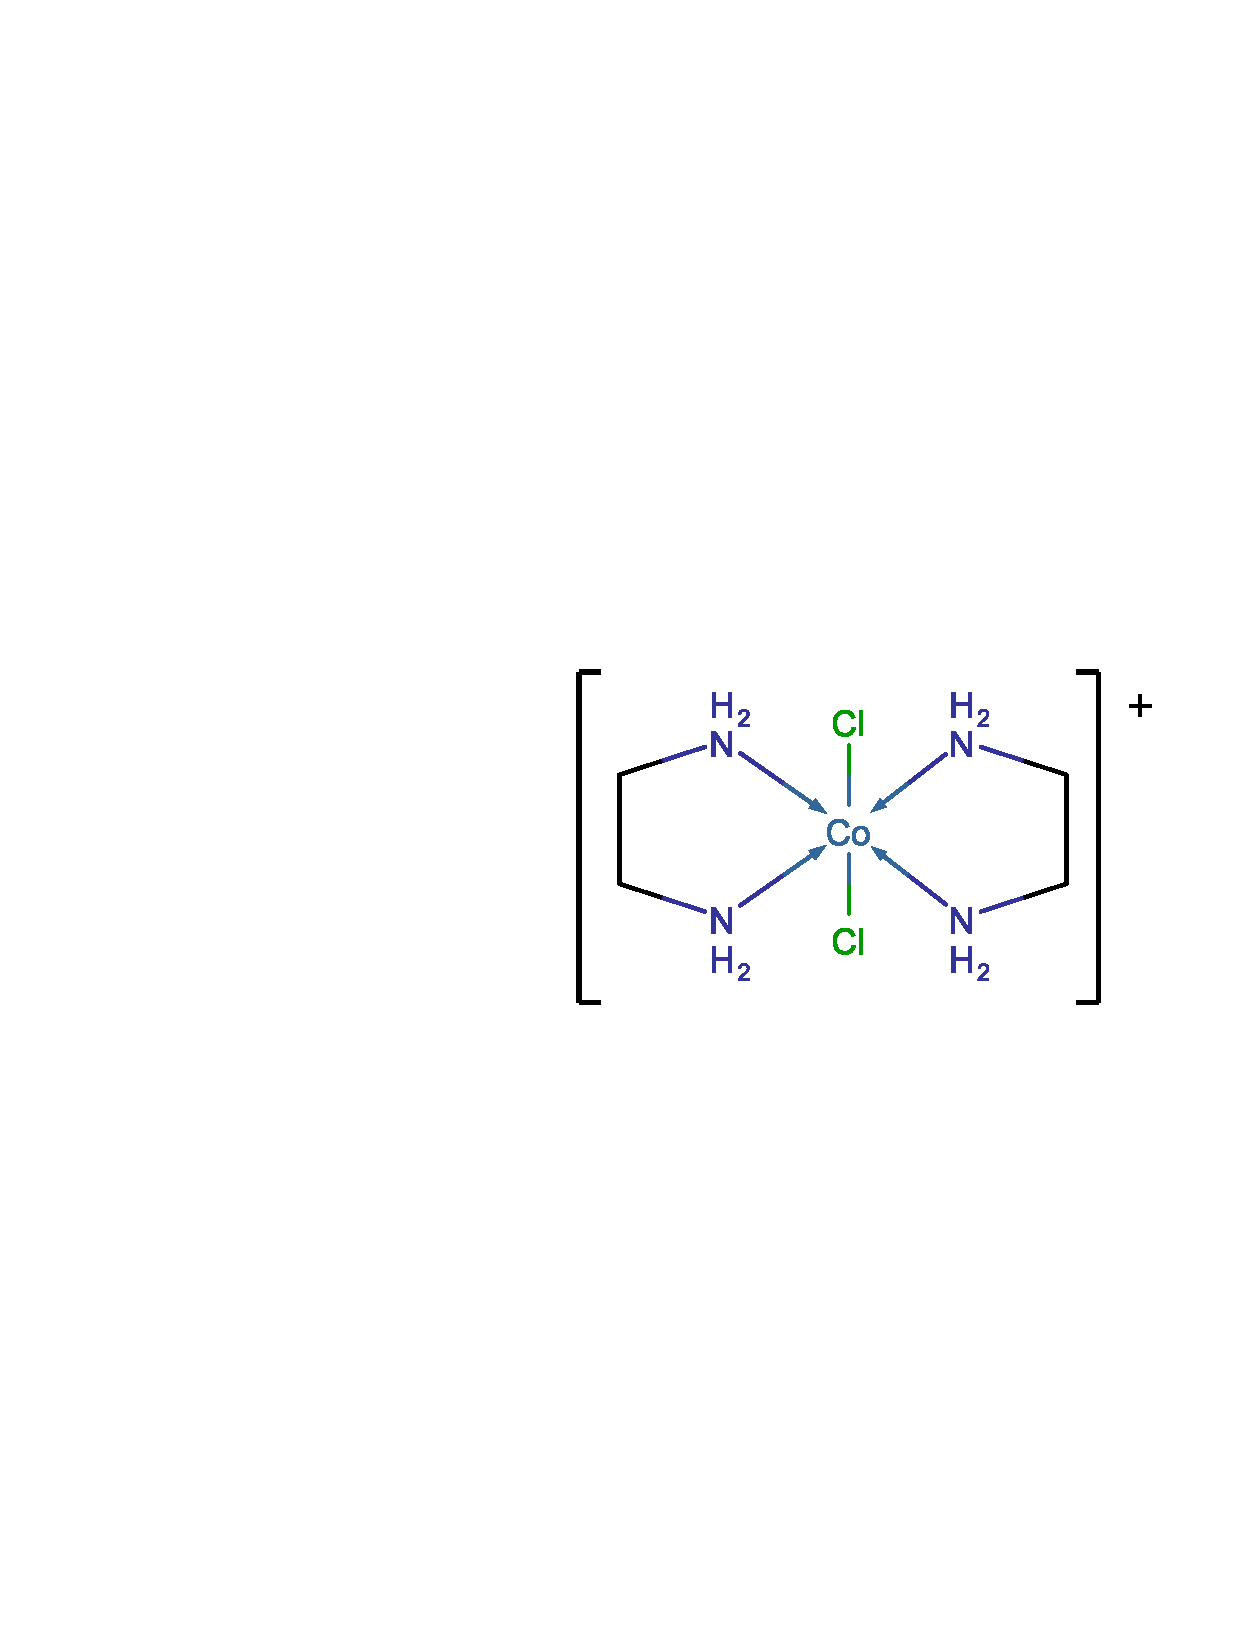
\includegraphics[width=0.45\linewidth]{images/trans.pdf} & 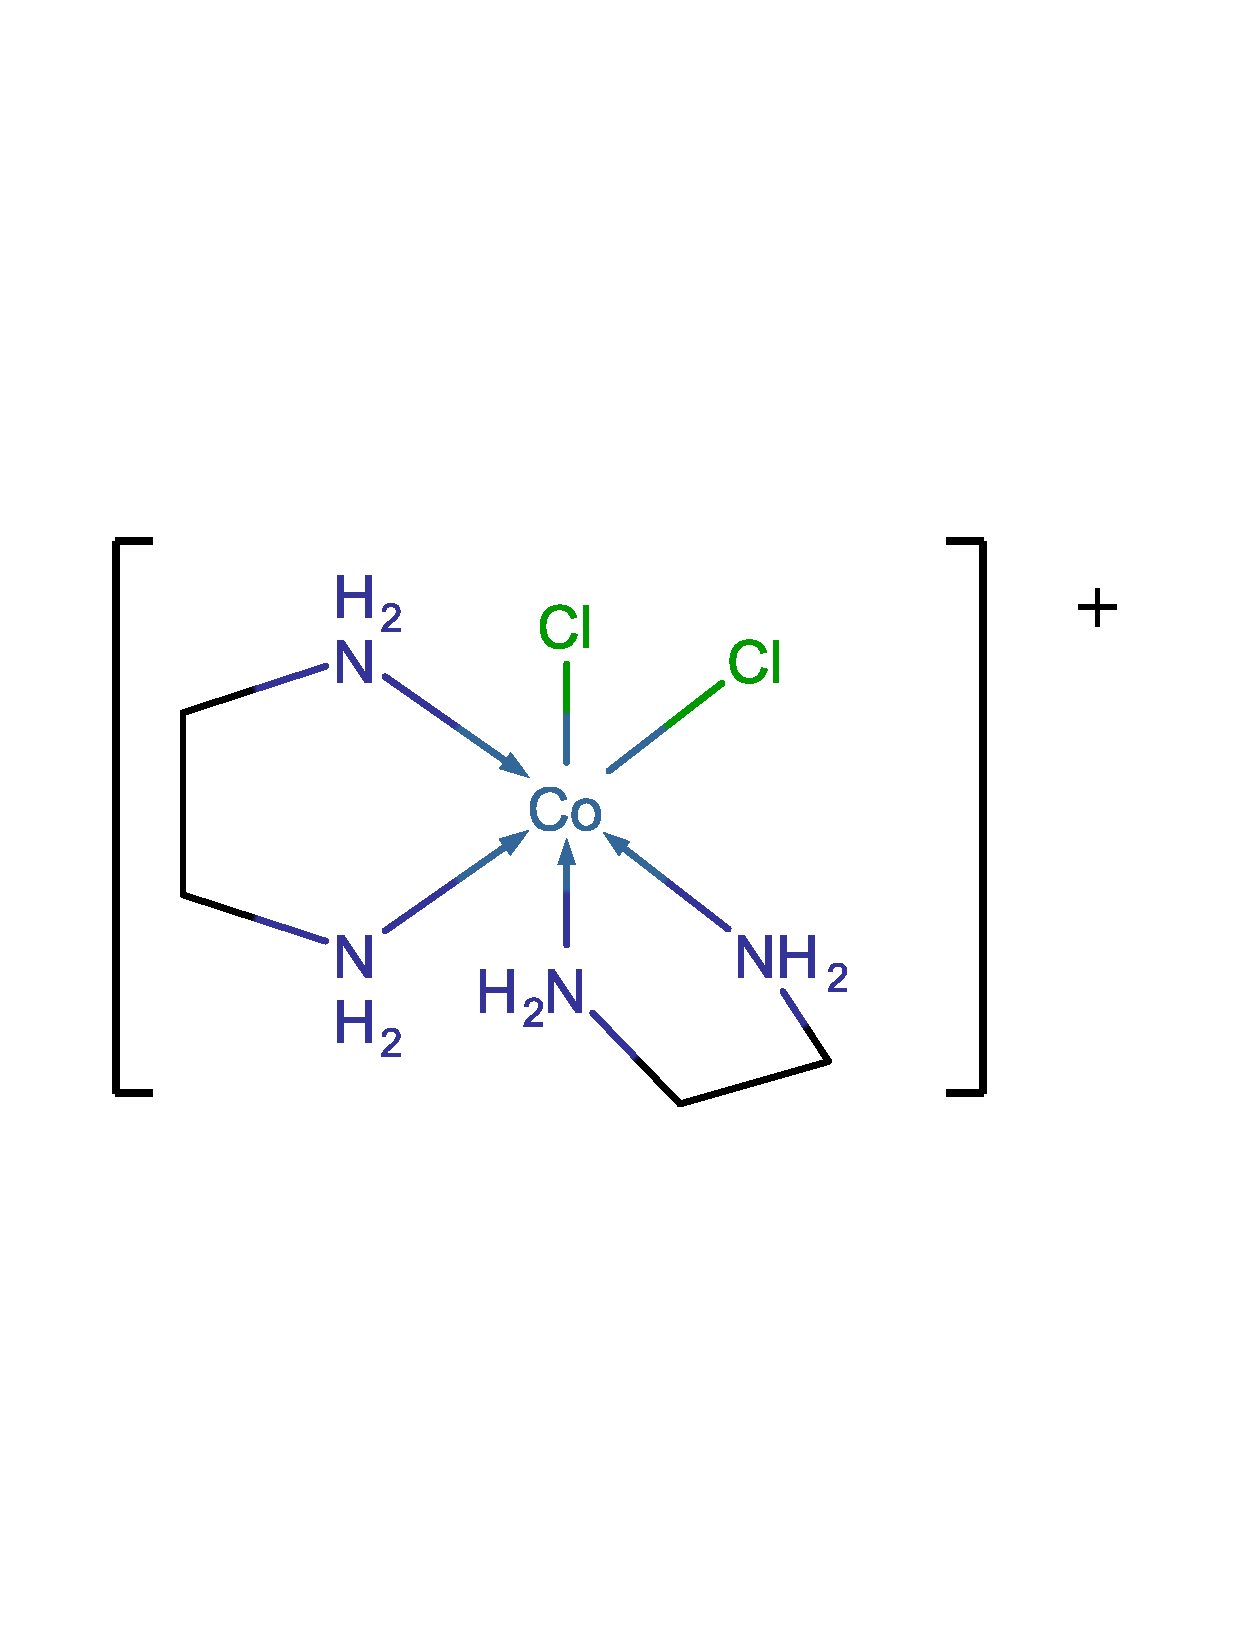
\includegraphics[width=0.45\linewidth]{images/cis.pdf} \\
        \end{tabular}
        \caption{Is\'omeros del cloruro de diclorobis (etilendiamina) cobalto(III), a la izquierda el trans.}
        \label{sch:my_label}
    \end{scheme}
    
	\section{Metodolog\'ia}
	Se pretendía sintetizar los dos isomeros (cis y trans) del compuesto diclorobis(etilendiamin)cobalto(III) por lo que se preparó el compuesto  trans y a partir de este se obtiene el producto cis. 
	Para tener el compuesto trans se mezclaron 4,2 mmol de $\ce{CoCl_{2}\cdot}\ce{6H_{2}O}}$ con 7 mL de $\ce{H_{2}O}$ y 3,5 mL de una solución al $\ce{10\%}$ de etilendiamina en agua en un tubo con desprendimiento lateral de forma tal que fue posible reducir la presión de la reacción para mantener un flujo constate de oxigeno, adicionalmente se pone la muestra en baño de maria durante una hora y se le adiciona una trampa fría en el camino entre el tubo de reacción y la bomba, para evitar el paso de cualquier sustancia hacia la misma.Se detuvo la bomba por unos instantes para agregar algunas gotas de de HCl concentrado y se agitó vigorosamente. Se mantuvo el vació hasta que dio inicio la precipitación de los cristales y en ese momento el tubo se introdujo en un baño de hielo, se filtró  y se lavaron los cristales con metanol que al pasar por la muestra se tiño de un violeta intenso que era sin duda cobalto sin reaccionar, posteriormente se probo el lavado con éter pero este disolvía el producto por lo que no se realizo. Por ultimo para obtener el producto final se calienta el  producto sobre un vidrio de reloj a $\ce{110^\circ}C$ durante una hora y media para obtener el trans-diclorobis(etilendiamin)cobalto(III).
	
	Para la obtención del producto cis se toma una fracción del trans en un vidrio del reloj, se deja en reposo durante 10 minutos en agua y posteriormente se calienta hasta la sequedad.

	\section{Resultados y Discusi\'on}
	En la s\'intesis de ambos productos fue posible observar la formaci\'on de un complejo con color rojo intenso. En el primer caso se debe a la reducci\'on del Co(II) al cobalto(III) en soluci\'on ac\'idica con presencia de ox\'igeno en el medio \cite{Afzal}.
	\begin{equation}
	    \ce{4 CoCl_2 + 4HCl + O_2(g) <=> 4CoCl_3 + 2H_2O}
	\end{equation}
	
	La reacci\'on anterior tiende hacia la izquierda, debido a que el cobalto (III) se hidroliza con facilidad. Sin embargo, usando el principio de Le Châtelier al burbujear constantemente ox\'igeno en la soluci\'on se consigue que la reacci\'on se desplace hacia la derecha. El cloruro de cobalto (III) en presencia de etilendiamina es quelado dando lugar al cloruro de diclorobis (etilendiamina) cobalto(III). La reacci\'on es posible debido a la afinidad del cobalto (III) por bases duras seg\'un el concepto de Pearson.
	\begin{equation}\label{eq: trans}
	    \ce{CoCl_3 + 2(en) -> [Co(en)2Cl_2]Cl}
	\end{equation}
	
	El complejo trans se caracteriza por su coloraci\'on verdosa, en la \autoref{tab: rendimientos} se puede observar un rendimiento del 67.3 \% para la reacci\'on anterior. 
	\begin{table}[h]
	    \centering
	    \caption{Rendimientos obtenidos para los dos is\'omeros.}
	    \begin{tabular}{c|cc}
	        \hline
	        & \textit{trans} & \textit{cis} \\
	        \hline
	        Recuperaci\'on (g) & 0.673 & 0.283 \\
	        Rendimiento & 67.3 \% & 85.4 \% \\
	        \hline
	    \end{tabular}
	    \label{tab: rendimientos}
	\end{table} 
	
	La segunda coloraci\'on roja se observa al disolver parte del complejo trans en agua, sobre la cual se obtiene la hidr\'olisis del mismo. El mecanismo de reacci\'on puede seguir dos rutas distintas, una asociativa y una disociativa \cite{Afzal}.
	\begin{equation}\label{eq: asociativa}
	    \small
	    \begin{array}{c}
	        \ce{[Co(en)_2Cl_2]+ + H_2O -> [Co(en)_2(H_2O)Cl_2]+} \\
	        \ce{[Co(en)_2(H_2O)Cl_2]+ -> [Co(en)_2(H_2O)Cl]^{2+} + Cl-}
	    \end{array}
	    \normalsize
	\end{equation}
	
	En la reacci\'on asociativa (\autoref{eq: asociativa}) una mol\'ecula de agua es coordinada por el centro met\'alico dando lugar a un complejo cobalto con n\'umero de coordinaci\'on 5, seguido de la posterior disociaci\'on de un \'atomo de cloro.
	\begin{equation}\label{eq: disociativa}
	    \begin{array}{c}
	        \ce{[Co(en)_2Cl_2]+ -> [Co(en)2Cl]^{2+} + Cl-} \\
	        \ce{[Co(en)_2Cl]^{2+} + H2O -> [Co(en)2(H2O)Cl]^{2+}}
	    \end{array}
	\end{equation}
	
	Lo anterior sugiere la existencia de un intermediario hidratado en la \autoref{eq: trans} responsable de la misma coloraci\'on rojiza de la s\'intesis del complejo cis. Al secar el complejo con ebulluci\'on se obtiene un compuesto de coloraci\'on an\'aloga a la del trans, raz\'on por la cual se cree que no se obtuvo el complejo cis, el cual presenta una coloraci\'on violeta \cite{Color}. 
	
	En 2014 fue determinado que el mecanismo de isomerizaci\'on cis-trans constituye una reacci\'on de primer orden, dependiente de la fuerza iónica de la solución dados las especies e intermediarios iónicos y el mecanismo favorecido por el solvente presente en la reacción sea $\ce{SN_{1}}$ o $\ce{SN_{2}}$ \cite{Mechanism}. El mecanismo se muestra en el \autoref{sch: isomerizacion}. En el se puede observar el seguimiento de una ruta disociativa adem\'as de la ausencia de intermedios acuosos. En ese sentido el mecanismo arroja una luz sobre la no obtenci\'on del complejo cis. La hidr\'olisis mostrada en la \autoref{eq: asociativa} y \autoref{eq: disociativa} ocurre \'unicamente en medios \'acidos \cite{Afzal}, por lo cual es posible que el cristal de \ce{[Co(en)_2Cl_2]Cl} contuviera remanentes de HCl provenientes de la s\'intesis, que en ultimas hubieran conducido la reacci\'on hacia la hidr\'olisis y no la isomerizaci\'on.
	\begin{scheme}[h]
	    \centering
	    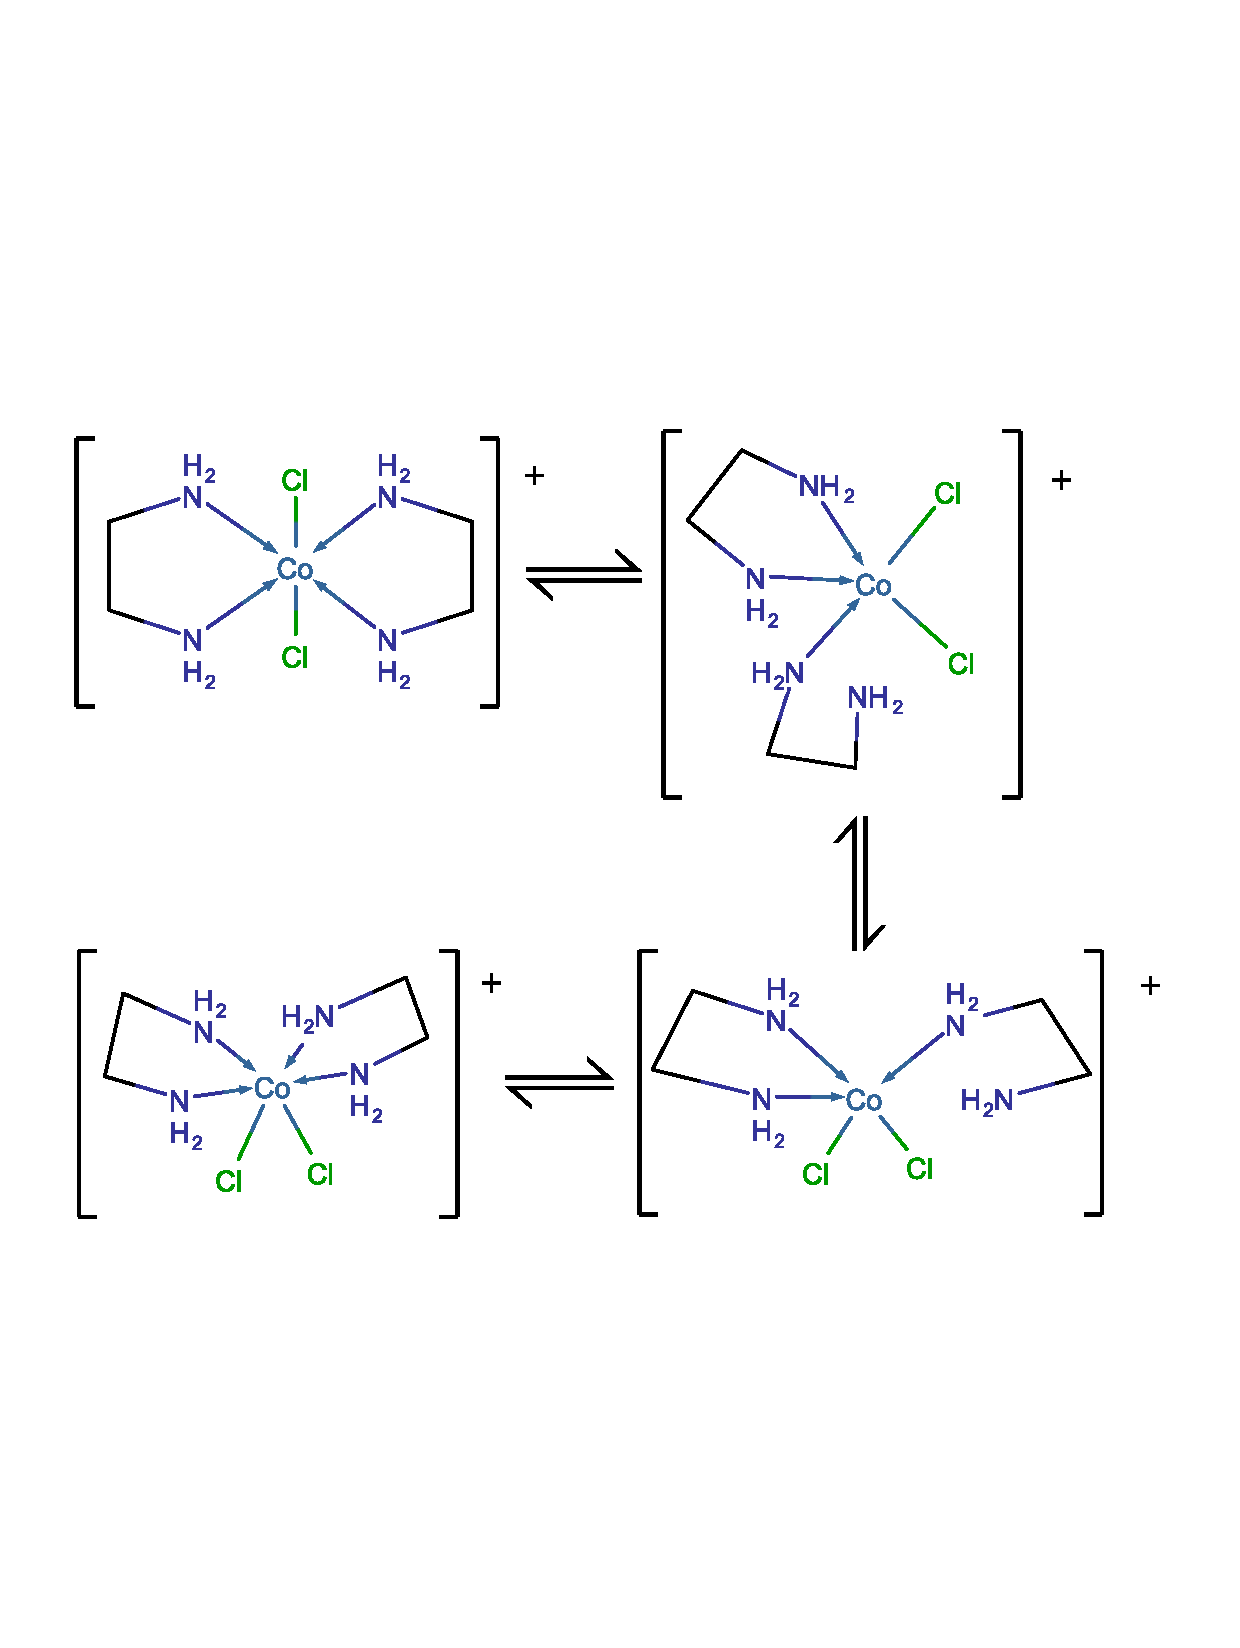
\includegraphics[width = \linewidth]{images/Isomerization.pdf}
	    \caption{Isomerizaci\'on cis-trans \cite{Mechanism}.}
	    \label{sch: isomerizacion}
	\end{scheme}
	
	\section{Preguntas}
	\subsection[Diferentes is\'omeros]{?`Cu\'antos diferentes is\'omeros existen de complejos que tienen la f\'ormula \ce{MA3B3}. Dib\'ujelos y n\'ombrelos.}
	Los isomeros que se obtiene por el llamado metodo de bailar o analizando todas las combinaciones posbiles son 2 y estos no cuentan con enantiomeros  dado que sus imagenes especulares representa el mismo compuesto.
	\begin{scheme}[h]
	    \centering
	    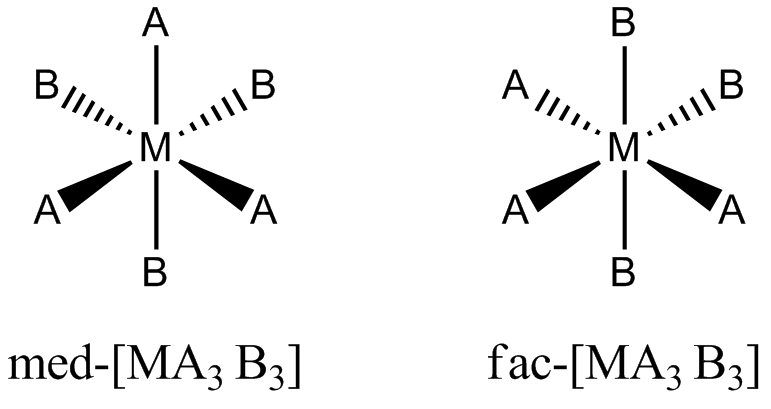
\includegraphics[width = 0.65 \linewidth]{images/isomeros.png}
	    \caption{Isomeros para un compuesto de forma $\ce{[MA_{3}B_{3}]}$.}
	    \label{sch: isomemeros}
	\end{scheme}
	
	\subsection[Elementos de simetr\'ia]{Determine los elementos de simetr\'ia para los is\'omeros cis y trans preparados en este experimento y asigne a los is\'omeros grupos puntuales.}
	El isómero trans tiene los siguientes elementos de simetría: E, $\ce{C_{2}}$ que contiene a los dos ligandos cloruro, $\ce{2C_{1}}$ por cada eje adicional en el octaedro y un plano perpendicular al eje de simetría principal que contiene a los dos ligando etilendiamina por lo que pertenece al grupo $\ce{D2h}$. Ahora el isómero cis tiene un eje de simetria principal del tipo $\ce{C_{2}}$ por lo que pertenece a este grupo \cite{iso}.
	\subsection[En vez de ox\'igeno]{En vez de ox\'igeno como agente oxidante se podr\'ia usar tambi\'en el per\'oxido de hidr\'ogeno en esta reacci\'on. Balancear la siguiente reacci\'on redox utilizando este reactivo:}
	\begin{equation}
	    \ce{Co^{2+} + H+ + H2O2 -> Co^{3+} + H2O}
	\end{equation}
	Se debe considerar que la prsencia de un agente oxidante en la solución favorece el desplazamiento del equilibrio hacia la dirección deseada por lo que usando peroxido se deben obtener mejores rendimientos. Ahora la ecuación balanceada será:
	\begin{equation}
	    \ce{Co^{2+} + 2H+ + H2O2 -> Co^{3+} + 2H2O}
	\end{equation}
	Sin embargo se debe considerar que este se debe encontrar en proporción estequiometrica, otras formas de acuerdo a la literatura de obtener mejores rendimientos es partir de sales de cobalto diferentes como carbonatos.
	\subsection[Ausencia de etilendiamina]{En la ausencia de la etilendiamina, el ion hexacuocobalto(III) reacciona r\'apidamente con agua seg\'un la reacci\'on siguiente, balancear la ecuaci\'on y determine el reactivo reductor.}
	\small
	\begin{equation}
	    \ce{[Co(H2O)6]^{3+} + H2O -> [Co(H2O)2]^{2+} + O2 + H+}
	\end{equation}
	Al balancear la ecuación se obtiene:
		\small
	\begin{equation}
	    \ce{[Co(H2O)6]^{3+} + 2H2O -> [Co(H2O)2]^{2+} + 3O2 + 12H+}
	\end{equation}
	Donde el cobalto y el oxigeno son reducidos y el hidrogeno se oxida, actuando pues este mismo como agente reductor. 
	Y esto ocurre en la ausencia de etilendiamina puesto que esta era la base de lewis que estabilizaba el metal en su estado (III).
	 
	\normalsize
	
	\section{Conclusiones}
    La reacción del síntesis del compuesto \newline diclorobis(etilendiamin)cobalto(III) que es de primer orden y la isomería que es dependiente cínicamente de factores como el disolvente y la concentración de iones puede favorecer la obtención tanto el isómero cis como el isómero trans, sin embargo dada la posibilidad de sustituir los iones cloruro por moléculas de agua u otros compuestos que puedan actuar como ligandos donores $\ce{\sigma}$ en la esfera de coordinación interna, se complica la conversión entre los isómeros llevando durante este proceso a producto estables no deseados. Los isómeros cis y trans del compuesto son estables en su forma cristalina. Durante la formación del isómero cis a patir del compuesto trans  aunque no se alcanza una coloración violeta en el producto final se torna opaco dada una ligera conversión entre una especie y otra. Los compuestos de cobalto (III) serán octaédricos.
	\phantomsection
	\bibliographystyle{unsrt}
	\begin{thebibliography}{9}
        \bibitem{cotton}
        Cotton A, Wilkinson G. Química inorganica avanzada. Primeda ed. Mexico: Limusa-Wiley; 1969. 1184 p. 
	    \bibitem{Afzal}
	    Afzal, D.; Baughman, R. G.; Ervin, H. D.; Moody, A. E.; Wohlers, H. D.; McCornick, J. M. Synthesis and Characterization of Coordination Compounds. \textit{Truman State University} \textbf{2014}.
	    \bibitem{Color}
	    Geometrical Isomers: cis & trans Isomers of Dichlorobis(ethylenediamine)cobalt(III) Chloride. \textit{UMass-Amherst} \textbf{2007}.
	    \bibitem{Mechanism}
	    Jacewicz, D.; Pranczk, J.; Wyrzykowski, D.; Żamojć, K.; Chmurzyński, L. Thermal properties of \ce{[Co(en)2Cl2]Cl} in solid state. Cis–trans isomerization of the \ce{[Co(en)2Cl2]+} complex ion in methanol. \textit{Reaction Kinetics, Mechanisms and Catalysis}. DOI: 10.1007/s11144-014-0742-y. Published Online: July 17, 2014, \textit{113} (2), 321–331.
	    \bibitem{iso}
	    Teoría de grupos de simetria. Available from: http://es.webqc.org/symmetrypointgroup-d2h.html
	\end{thebibliography}
\end{document}
